\documentclass[french]{article}
\usepackage[utf8]{inputenc}
\usepackage[T1]{fontenc}
\usepackage{babel}
\usepackage{url}

\usepackage{pdfpages}
\usepackage{framed}
\usepackage{hyperref}
\usepackage{graphicx}
\usepackage{ulem}
\usepackage{adjustbox}
\usepackage{blindtext}
\usepackage{tocbibind}
\usepackage[toc,page]{appendix}
\PassOptionsToPackage{hyphens}{url}

\usepackage{minted}

\title{Face recognition with convoluted neural networks
\\-
\\OT1-PJ12}
\author{FOSSART Alexis, RENAULT Benoit}
\date{January 31st 2018}

%% Margins
\usepackage[
    top=3cm,
    bottom=3cm,
    left=3cm,
    right=3cm
]{geometry}

\begin{document}

\maketitle

\medskip

\tableofcontents

\newpage

\section{Introduction}

\paragraph{} This document describes all of the work we've done for the INSA 5IF Deep Learning Project - CNNs for Face Recognition.

\paragraph{} In the first part, we provide instructions as to where to find our source code as well as how to run it.

\paragraph{} In the second part we describe our entire workflow, providing a highly detailed and commented code.

\paragraph{} Finally, we conclude on our overall work, what it brought us, and how we could have improved it.

\section{Running the project}

\subsection{Prerequisites}

Please run it preferably on a GNU/Linux distribution. You should also have installed the latest version available to you of Git and Docker (google them to find their installation instructions for your OS).

\subsection{Quickstart}

\paragraph{} Clone this repository:

\begin{minted}{bash}
\$ git clone
\end{minted}

\paragraph{} Run the build.sh, then start\_jupyter, both with sudo rights if you haven't set your user so that you can use docker commands without being root.

\begin{minted}{bash}
\$ sudo ./build.sh
\$ sudo ./start_jupyter.sh
\end{minted}

\paragraph{} The first command log should end with a message like the following:

\begin{minted}{bash}
Successfully built 554f78aa2d91
Successfully tagged deep:latest
\end{minted}

\paragraph{} The second one should return something like:

\begin{minted}{bash}
52aac7bf9976a85dd9b98258dc350bbe790acb94152c33884f6b3885a21bf31a
\end{minted}

\paragraph{} You can check whether the container started properly by writing:

\begin{minted}{bash}
\$ sudo docker ps -a
\end{minted}

\paragraph{} If everything is fine you should get a line like the following (what matters here is that the "STATUS" field is "UP"):

\begin{minted}{bash}
CONTAINER ID        IMAGE               COMMAND                  CREATED       
52aac7bf9976        deep                "/bin/sh -c 'jupyter…"   13 minutes ago
STATUS                    PORTS                    NAMES
Up 13 minutes             0.0.0.0:8887->8888/tcp   deep_jupyter
\end{minted}

\paragraph{} Once this is done, you should have a "data" folder in your cloned repository. Copy the test\_images and train\_images data folders into it. Then open a bash in the container :

\begin{minted}{bash}
\$ sudo docker exec -it deep_jupyter /bin/bash
\end{minted}

\paragraph{} And run the following commands inside to build the image database :

\begin{minted}{bash}
\$ cd data

\$ /opt/caffe/build/tools/convert_imageset --shuffle --gray
train_images/ posneg.txt train_lmdb

\$ /opt/caffe/build/tools/convert_imageset --shuffle --gray
test_images/ testposneg.txt test_lmdb

\$ /opt/caffe/build/tools/compute_image_mean train_lmdb/ train_mean.binaryproto

\$ /opt/caffe/build/tools/compute_image_mean test_lmdb/ test_mean.binaryproto
\end{minted}

\paragraph{} You can then close your terminal and open your favorite web browser to \url{http://localhost:8887/} . This will open the Jupyter Notebook instance that is inside the container.

\paragraph{} You will get to a login form. In the "Password or token" field, enter "demo". You will then be redirected to the usual Jupyter Notebook interface. Open the "notebooks" folder, and then the "01\_CNN\_Training.ipynb" if you want to train the neural network, "02\_CNN\_Usage.ipynb" if you want to test a pre-trained one or your own, or "03\_CNN\_Image\_Parsing.ipynb" if you wish to use the neural network to detect faces in a given set of images.

\newpage

\section{Description of the work}

\subsection{Setting up Caffe to be used through PyCaffe and Docker}

\paragraph{} We chose to use Docker to run Caffe, in order to avoid the dependency hell that it is to install it by hand. First, with the help of the \href{https://github.com/BVLC/caffe/tree/master/docker
}{Official Caffe Docker Image}, and \href{https://towardsdatascience.com/playing-with-caffe-and-docker-to-build-deep-learning-models-99c9570ffc3d}{this article}, we had it run aside an IPython Notebook, in order to ease the development process, especially for the graphical side. This still took quite a few hours considering that some of the article's information was kind of misleading.

\paragraph{} We then took a few hours to freely roam about the \href{http://caffe.berkeleyvision.org/tutorial/}{Official Caffe Tutorial} and \href{http://christopher5106.github.io/deep/learning/2015/09/04/Deep-learning-tutorial-on-Caffe-Technology.html}{this other tutorial} to try and get to know the tool.

\subsection{Training the network}

\paragraph{} We then set out on trying to train our own neural network thanks to the provided configuration files, and it took quite a bit of trial and error to get this all to work together, ending with the following little snippet of code.

\subsubsection{Code}

\begin{minted}{python}
import numpy as np
import matplotlib.pyplot as plt
from PIL import Image
import caffe

caffe.set_mode_cpu()
solver = caffe.SGDSolver('solver.prototxt')
solver.solve()
\end{minted}

\subsubsection{Adjusting the Docker image for better performances during training}

\paragraph{} Since we had no compatible GPU, and had to use the CPU version of Caffe, we very soon realized while training the network that it only used one core of our CPUs by default taking one entire hour to create the network with only 50000 iterations. After much research and hazardous tries (mostly following more or less outdated StackOverflow like \href{https://stackoverflow.com/questions/31395729/how-to-enable-multithreading-with-caffe}{this one}), we eventually stumbled upon the \href{https://github.com/intel/caffe}{Intel Caffe} fork of the software, optimized for, you guessed it, Intel CPUs, and allowing the to set at build time the maximum number of threads to authorize for Caffe, therefore permitting us to use our CPUs to their fullest (it simply halved the training time).

\subsection{Evaluating the detection performance of our NN}

\paragraph{} After getting the network to train within a more reasonable time, we tried to evaluate its accuracy by using it against the same training data we originally used, then against the provided Google and Yale datasets.

For the basic provided network trained with 100 000 iterations, we got an accuracy of 0.956450628053 for the training set, and an accuracy of 0.282731681034 for the Google and Yale datasets (which is pretty bad since a random guess of whether the image would be better).

\subsubsection{Code}

\paragraph{Basic setup of neural network}

\begin{minted}{python}
import caffe

caffe.set_mode_cpu()

model_train = 'conv.prototxt'
model_test = 'deploy.prototxt'
weights = 'deep_iter_100000.caffemodel'

net_training = caffe.Net(model_train, weights, caffe.TEST)
net_testing = caffe.Net(model_test, weights, caffe.TEST)
\end{minted}

\paragraph{Compute the accuracy of the previously trained neural network on the training dataset (see 01\_CNN\_Training notebook) by using the accuracy layer of the network (defined in conv.prototxt)}

\begin{minted}{python}
NUMBER_OF_IMAGES_ON_TRAINING_SET_WITHOUT_FACE = 26950
NUMBER_OF_IMAGES_ON_TRAINING_SET_WITH_A_FACE = 64770

TOTAL_NUMBER_OF_IMAGES_ON_TRAINING_SET = (NUMBER_OF_IMAGES_ON_TRAINING_SET_WITHOUT_FACE +
                                          NUMBER_OF_IMAGES_ON_TRAINING_SET_WITH_A_FACE)

total_accuracy = 0
batch_size = net_training.blobs['data'].num
test_iters = TOTAL_NUMBER_OF_IMAGES_ON_TRAINING_SET / batch_size

for i in range(test_iters):
    net_training.forward()
    batch_accuracy = net_training.blobs['accuracy'].data
    total_accuracy += batch_accuracy
accuracy = total_accuracy / test_iters

print "Accuracy of trained network on train data: {}".format(accuracy)
print "Number of well classified images on train data: {}".format(
    int(accuracy * TOTAL_NUMBER_OF_IMAGES_ON_TRAINING_SET))
\end{minted}

\paragraph{Evaluate the accuracy of the previously trained neural network on the test dataset}

\begin{minted}{python}
NUMBER_OF_IMAGES_ON_GOOGLEFACE_TEST = 632
NUMBER_OF_IMAGES_ON_GOOGLE_IMAGES = 6831
NUMBER_OF_IMAGES_ON_YALEFACES_TEST = 165

TOTAL_NUMBER_OF_IMAGES_ON_TEST_SET = (NUMBER_OF_IMAGES_ON_YALEFACES_TEST +
                                      NUMBER_OF_IMAGES_ON_GOOGLE_IMAGES +
                                      NUMBER_OF_IMAGES_ON_GOOGLEFACE_TEST)

img_classified_as_faces = 0
img_classified = 0

total_accuracy = 0

batch_size = net_testing.blobs['data'].num
test_iters = TOTAL_NUMBER_OF_IMAGES_ON_TEST_SET / batch_size

for i in range(test_iters):
    net_testing.forward()
    batch_accuracy = net_testing.blobs['accuracy'].data
    total_accuracy += batch_accuracy
    for i in range(batch_size):
        img_classified += 1
        if net_testing.blobs['prob'].data[i].argmax():
            img_classified_as_faces += 1
            

accuracy = total_accuracy / test_iters

print "Number of faces found on test : {} / {} images".format(img_classified_as_faces,
                                                              img_classified)
print "Accuracy of trained network on test data: {}".format(accuracy)
print "Number of well classified images on test data: {}".format(
    int(accuracy * TOTAL_NUMBER_OF_IMAGES_ON_TEST_SET))
\end{minted}

\subsection{Implementing a naive face detector}

\paragraph{} Nevermind our previous results, we set out to produce a basic naive face detector algorithm, described below.

\paragraph{Basic setup of neural network}

\begin{minted}{python}
import numpy as np
import matplotlib.pyplot as plt
from PIL import Image
import cv2
import caffe
import os

caffe.set_mode_cpu()
model = 'deploy.prototxt'
weights = 'deep_iter_100000.caffemodel'
net = caffe.Net(model, weights, caffe.TEST)

try:
    os.mkdir("../data/results/")
except OSError: pass
try:
    os.mkdir("../data/results/1/")
except OSError: pass
\end{minted}

\paragraph{Implementation of face detector} The downscaling is done by factor of 2 (using an integrated function of opencv which seems to be the only way to do pyramid scaling without destroying the quality of the images we could find). This is a naive algorithm implementation, without heuristics : we simply used a shifting window of size 36*36px and offset 4px.

\begin{minted}{python}
for id_img in range(1, 8):
    # Used on 7 images named 1.jpg to 7.jpg
    image_path = '../data/' + str(id_img) + '.jpg'
    
    # Open image and convert to gray scale
    im =  cv2.imread(image_path)
    im = cv2.cvtColor(im, cv2.COLOR_BGR2GRAY)
    
    # Save base image for future comparison
    imbase = im
    
    scale = 1
    
    base_save_path = "../data/results/"
    img_base_name = str(id_img) + "_"
    
    # Used to batch save detected faces, and avoid writing to disk at every loop
    keep = dict()
    
    # Tuple with (width, height)
    shifting_window_size = 36, 36
    offset = 4
    
    min_probability_for_a_match = 0.99
    
    while (len(im) >= shifting_window_size[0] * 2 and 
           len(im[0]) > shifting_window_size[1] * 2):
        # Downscale of the image using opencv pyramid scaling
        im = cv2.pyrDown(im)
        scale*=2
        
        img_scale_name = img_base_name + str(scale) + "_"
        
        display_image(im)
        
        # Face detector
        for x in range(0, len(im) - shifting_window_size[0], offset):
            for y in range(0, len(im[0]) - shifting_window_size[1], offset):
                img_name = img_scale_name + str(x) + "_" + str(y) + ".png"
                
                # Create the shift window image on the original scaled image 
                imtmp = np.array(im [x:x + shifting_window_size[0],
                                     y:y + shifting_window_size[1]])
                
                # Transform the data to be compatible as an entry to the neural network
                im_input = imtmp[np.newaxis, np.newaxis, :, :] / 256.0
                
                # Input the data in the NN
                net.blobs['data'].reshape(*im_input.shape)
                net.blobs['data'].data[...] = imtmp
                
                # Run the NN
                output = net.forward()
                
                # If the probability that the image that is in the
                #shift window is a face is higher than 99%
                if output['prob'][0][1] > min_probability_for_a_match:
                    # We add a bounding box in the original image
                    white = 255
                    for i in range (x * scale, (x + shifting_window_size[0]) * scale):
                        imbase[i][y * scale] = white
                        imbase[i][(y + shifting_window_size[1]) * scale] = white
                    for j in range(y * scale, (y + shifting_window_size[1]) * scale):
                        imbase[x * scale][j] = white
                        imbase[(x + shifting_window_size[0]) * scale][j] = white

                    # Save this in memory
                    save_dir = "1/"
                    save_path = base_save_path + save_dir + img_name
                    keep[save_path] = imtmp
    
    # When everything is done we show the original image
    #with the bounding boxes and save it as a file
    display_image(imbase)
    save_results = "../data/results/" + str(id_img) + ".jpg"
    cv2.imwrite(save_results, imbase)
    
    # We also save the face subimages we found to improve the NN in the future
    for path,img in keep.iteritems():
        cv2.imwrite(path, img)
\end{minted}

\subsection{Improving the results}

\paragraph{} From our previous experiments, we saw that our first phase of training conducted to a lot of false positives (see figures below). So we set out on a way to solve this.

\begin{figure}[h]
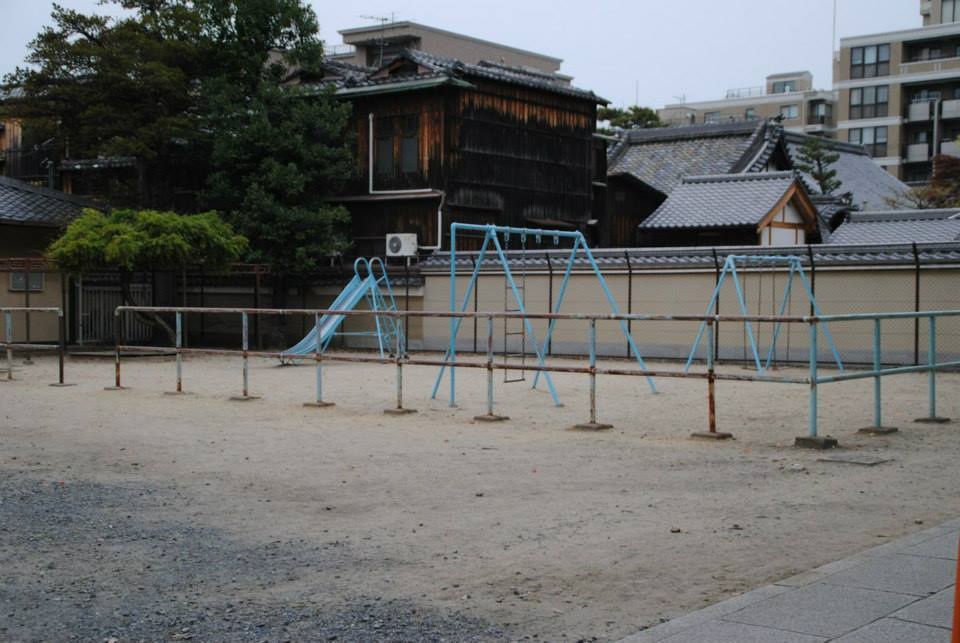
\includegraphics[height=5cm]{1.jpg}
\centering
\caption{One of the original images used, without faces}
\end{figure}

\begin{figure}[h]
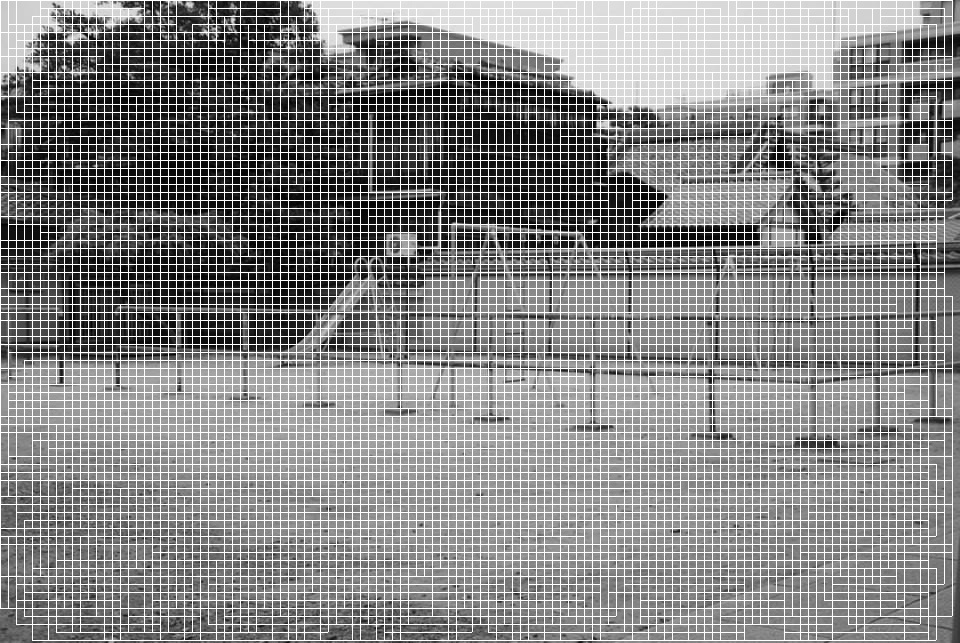
\includegraphics[height=5cm]{1_boxes.jpg}
\centering
\caption{Same image but with false positive bounding boxes}
\end{figure}

\paragraph{} With 7 images (since we had no time to run more than this, given the meager performance of our naive algorithm and the fact that we did not have an appropriate machine at our disposal) that we knew had no faces in them, we created a lot of false positives thumbnails and used them for training in the "no face" category (0 folder). To balance the greater number of negative images, we simply copy pasted the files in the positive images to match it.

\newpage

\section{Conclusion}

\paragraph{} Ideally, we would have to apply the same technique as in the last section : that is, using the NN on images we know that they contain no faces and feed the false positives to train the NN again and again.

\paragraph{} Eventually, we would get to playing with other NN configurations (which we had no time to, given the speed at which our tests were running), modifying the layers especially : their nature, complexity, quantity... Knowing that the convolution layers detect features that make a face : the more a convolution layer has elements, the more it will be able to detect different features (for example, if the first layer had only a single neuron, it would likely end up recognizing an oval shape, if it had two, it would probably detect two oval shapes,...).

\paragraph{} This was overall a pleasant experience in neural networks and deep learning, despite the fact that our machines and time availabilities did not allow us to go any further.

\end{document}
